\section{Auswertung}
	\label{sec:auswertung}

	Die Messung der Offsetspannung $U_0$ ergab:

	\begin{equation*}
		U_0 = \SI{0.02}{\milli\volt}.
	\end{equation*}

	W"ahrend des Versuchs kam es nicht zu Temperaturdrifts.
	Bei der Messung der Ansprechzeit ergab sich bereits nach $\SI{10}{\second}$ eine S"attigung, 
	weshalb wir auch f"ur die An\-sprech\-zeit $\SI{10}{\second}$ benutzt haben.

	Die Messung der Thermospannung der verschiedenen Oberfl"achen bei verschiedenen Temperaturen ergab die in den Tabellen \eqref{schwarz} bis \eqref{spiegel} gemessenen Werte. Eine lineare Regression der Werte ist in den Graphen \eqref{schwarz_graph} bis \eqref{spiegel_graph} zu erkennen.

	Dabei ergibt sich f"ur den fit mit $m*x+b$ folgende Werte mit $b = -0.1$:

	\begin{eqnarray}
		m &=& \SI{2.63 (3) e-10}{}\\
		m &=& \SI{2.60 (3) e-10}{}\\
		m &=& \SI{5.10 (35) e-11}{}\\
		m &=& \SI{2.64 (37) e-11}{}
	\end{eqnarray}

	\begin{center}
			\tiny{1: schwarz, 2: wei"s, 3: matt, 4: spiegelnd}
	\end{center}

	Aus dem Zusammenhang:

	\begin{eqnarray*}
		U &\propto& \epsilon\,\sigma\,T^4\\
		\Rightarrow \mathrm{const} &=& \frac{\epsilon\,\sigma\,T^4}{U},\\
		\Rightarrow \frac{\epsilon\,\sigma\,T^4}{U} &=& \frac{\epsilon_\mathrm{schwarz}\,\sigma\,T^4_\mathrm{schwarz}}{U_\mathrm{schwarz}},\\
		\epsilon_{schwarz} &=& 1,\\
		\Rightarrow \epsilon &=& \frac{T^4_\mathrm{schwarz}}{U_\mathrm{schwarz}} \frac{U}{T^4},\\
		m &=& \frac{U}{T^4},\\
		\Rightarrow \epsilon &=& \frac{m}{m_\mathrm{schwarz}},
	\end{eqnarray*}

	ergibt sich f"ur das Emissionsverm"ogen der einzelnen Oberfl"achen:

	\begin{eqnarray*}
		\epsilon_\mathrm{schwarz} &=& \SI{1}{}\\
		\epsilon_\mathrm{wei"s} &=& \SI{0.99 (4)}{}\\
		\epsilon_\mathrm{matt} &=& \SI{0.19 (5)}{EINHEIT}\\
		\epsilon_\mathrm{spiegelnd} &=& \SI{0.10 (5)}{EINHEIT}
	\end{eqnarray*}

	Der Fehler gergibt sich durch Gau"s'sche Fehlerfortpflanzung der Fehler bei $m$.
	Die Literaturwerte \cite{emission} weichen von diesen ab.
	So wird beispielsweise f"ur wei"s ein Ko\-ef\-fi\-zient von $0.90$ bis $0.95$ angegeben.
	Dies liegt wohl daran, dass wir die schwarze Fl"ache als schwarzen Strahler angenommen haben, was in wirklichkeit nicht v"ollig richtig ist.

	\begin{figure}[htbp]
		\centering
		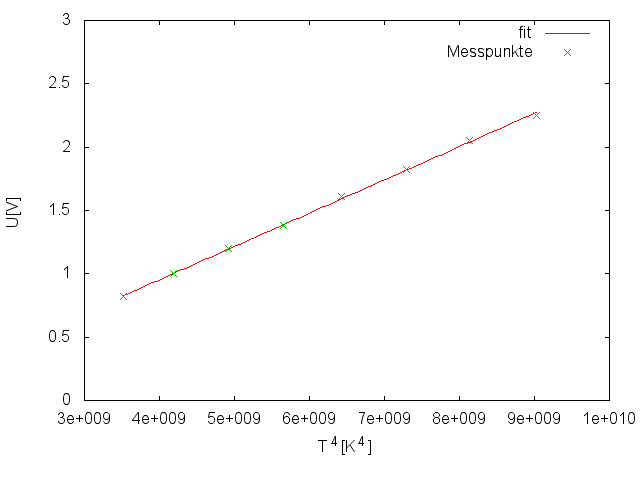
\includegraphics[width = 12cm]{img/schwarz.png}
		\caption{Thermospannung in Abh"angigkeit von der Temperatur bei der schwarzen Oberfl"ache}
		\label{schwarz_graph}

		\centering
		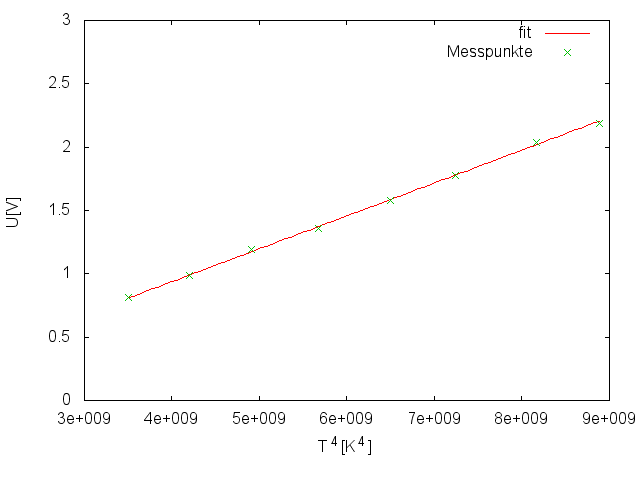
\includegraphics[width = 12cm]{img/weiss.png}
		\caption{Thermospannung in Abh"angigkeit von der Temperatur bei der wei"sen Oberfl"ache}
		\label{weis_graph}
	\end{figure}

	\begin{figure}[htbp]
		\centering
		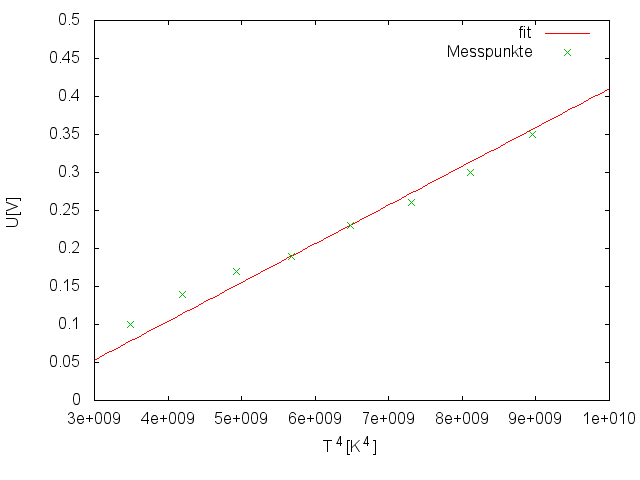
\includegraphics[width = 12cm]{img/matt.png}
		\caption{Thermospannung in Abh"angigkeit von der Temperatur bei der matten Oberfl"ache}
		\label{matt_graph}

		\centering
		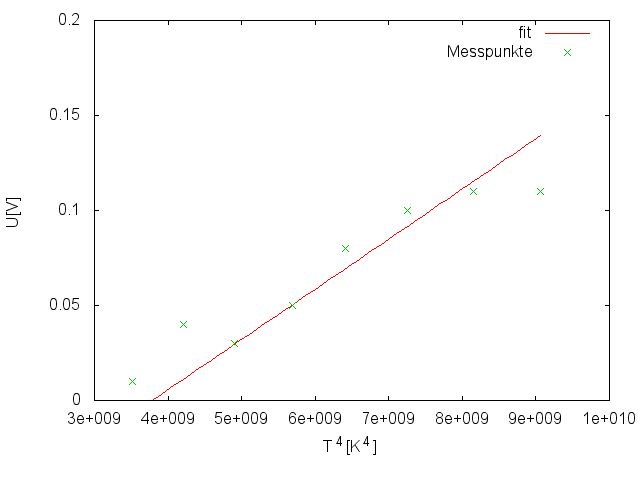
\includegraphics[width = 12cm]{img/spiegel.png}
		\caption{Thermospannung in Abh"angigkeit von der Temperatur bei der spiegelnden Oberfl"ache}
		\label{spiegel_graph}
	\end{figure}

	\begin{table}
\begin{center}
\begin{tabular}{r|r}
T[$^\circ$ C] & U[V] \\
\hline
84.8 & 2.25 \\
79.8 & 2.05 \\
74.9 & 1.82 \\
69.7 & 1.61 \\
64.8 & 1.38 \\
59.9 & 1.20 \\
54.8 & 1.00 \\
50.0 & 0.82 \\
\end{tabular}
\caption[Thermospannung]{Messung der Thermospannung einer schwarzen Oberfl"ache}
\label{schwarz}
\end{center}
\end{table}

	\begin{table}
\begin{center}
\begin{tabular}{r|r}
T[$^\circle$ C] & U[V] \\
84.0 & 2.19 \\
80.0 & 2.04 \\
74.6 & 1.78 \\
70.1 & 1.58 \\
64.9 & 1.36 \\
59.8 & 1.19 \\
54.9 & 0.99 \\
49.9 & 0.81 \\
\end{tabular}
\caption[Thermospannung]{Messung der Thermospannung einer wei"sen Oberfl"ache}
\label{weiss}
\end{center}
\end{table}

	\begin{table}
\begin{center}
\begin{tabular}{r|r}
T[$^\circle$ C] & U[V] \\
84.4 & 0.35 \\
79.7 & 0.30 \\
75.0 & 0.26 \\
70.0 & 0.23 \\
64.9 & 0.19 \\
60.0 & 0.17 \\
54.9 & 0.14 \\
49.8 & 0.10 \\
\end{tabular}
\caption[Thermospannung]{Messung der Thermospannung einer matten Oberfl"ache}
\label{matt}
\end{center}
\end{table}

	\begin{table}
\begin{center}
\begin{tabular}{r|r}
T[$^\circle$ C] & U[V] \\
85.0 & 0.11 \\
79.9 & 0.11 \\
74.7 & 0.10 \\
69.6 & 0.08 \\
65.0 & 0.05 \\
59.8 & 0.03 \\
55.0 & 0.04 \\
50.0 & 0.01 \\
\end{tabular}
\caption[Thermospannung]{Messung der Thermospannung einer spiegelnden Oberfl"ache}
\label{spiegel}
\end{center}
\end{table}


	Eine nicht lineare Regression der Messpunkte aus Tabelle \eqref{abstand} mit $m/(x+b)^2$ ergibt:

	\begin{eqnarray*}
		m = \SI{494.96 (6292)}{}\\
		b = \SI{11.38 (197)}{}
	\end{eqnarray*}

	Der $1/r^2$ Zusammenhang wird in Graphik \eqref{abstand_graph} damit graphisch sichtbar. Daf"ur haben wir den ersten Messwert rausgelassen, da dieser nicht richtig lag.

	\begin{figure}[htbp]
		\centering
		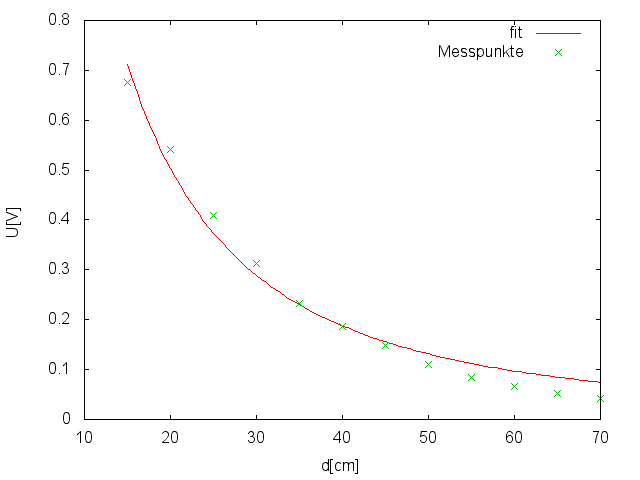
\includegraphics[width = 12cm]{img/abstand.png}
		\caption{Thermospannung in Abh"angigkeit vom Abstand}
		\label{abstand_graph}
	\end{figure}

	\begin{table}
\begin{center}
\begin{tabular}{c|c}
d[cm] & U[mV] \\
\hline
10 & 0.78 \\
15 & 0.68 \\
20 & 0.54 \\
25 & 0.41 \\
30 & 0.31 \\
35 & 0.23 \\
40 & 0.19 \\
45 & 0.15 \\
50 & 0.11 \\
55 & 0.08 \\
60 & 0.07 \\
65 & 0.05 \\
70 & 0.04 \\
\end{tabular}
\caption[Thermospannung]{Thermospannung einer wei"sen Oberfl"ache in Abh"angigkeit vom Abstand}
\label{abstand}
\end{center}
\end{table}

